Due to the large Monte Carlo modeling uncertainties of the top background at
high $\met$ observed in the analysis of the 2015 data (about 40\% in the signal
region for IM6) this process is estimated with a data-driven method in the
combined 2015 and 2016 data. To this end the Top control region ($\crtop$) is
introduced to estimate the contribution of $t \bar{t}$ and single top processes
in the signal region. In addition to cuts from A to H as defined in
\cref{sec:event-selection-1} the $\crtop$ region selects events with:
\begin{itemize}
\item Exactly one good muon.
\item No baseline electrons.
\item The transverse mass defined in \eqref{eq:99} of the $\met - \mu$ system
  satisfies $30 < m_\mathrm{\, T} < 100$~GeV compatible with a $W$ boson
  production.
\item At least one of the selected jets in the event is identified as a $b$-jet.
\end{itemize}
\cref{fig:top_plots} report the $\met$ and the leading jet $\pt$ distributions
after the background only fit described in
\cref{sec:glob-simult-likel,sec:fit-strategy}. It shows, within uncertainties, a
good agreement between data and \gls{mc}.
\begin{figure}[!th]
  \centering
  \begin{subfigure}[t]{.48\linewidth}
    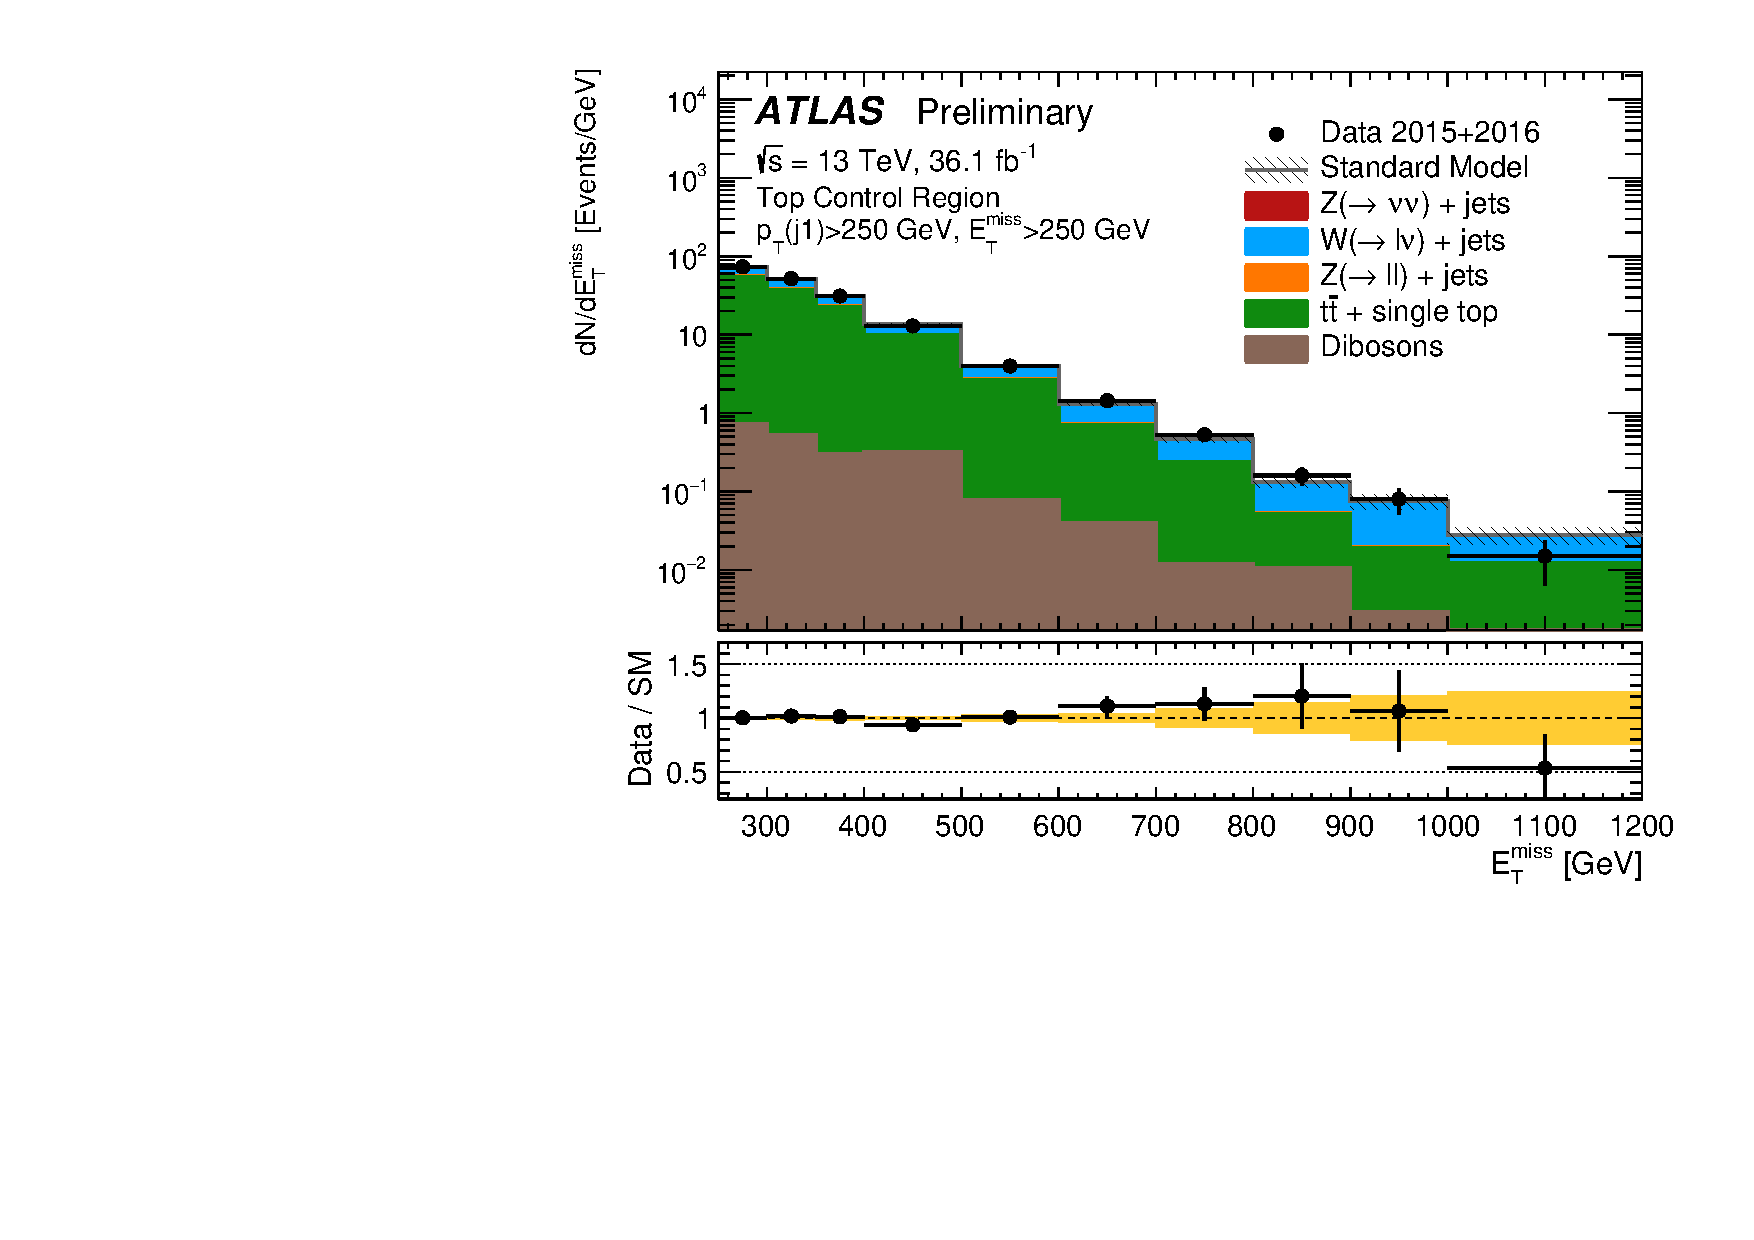
\includegraphics[width=\linewidth]{top_cr_met}
    \caption{$\met$ distribution.}
    \label{fig:top_cr_et_miss}
  \end{subfigure}
  \begin{subfigure}[t]{.48\linewidth}
    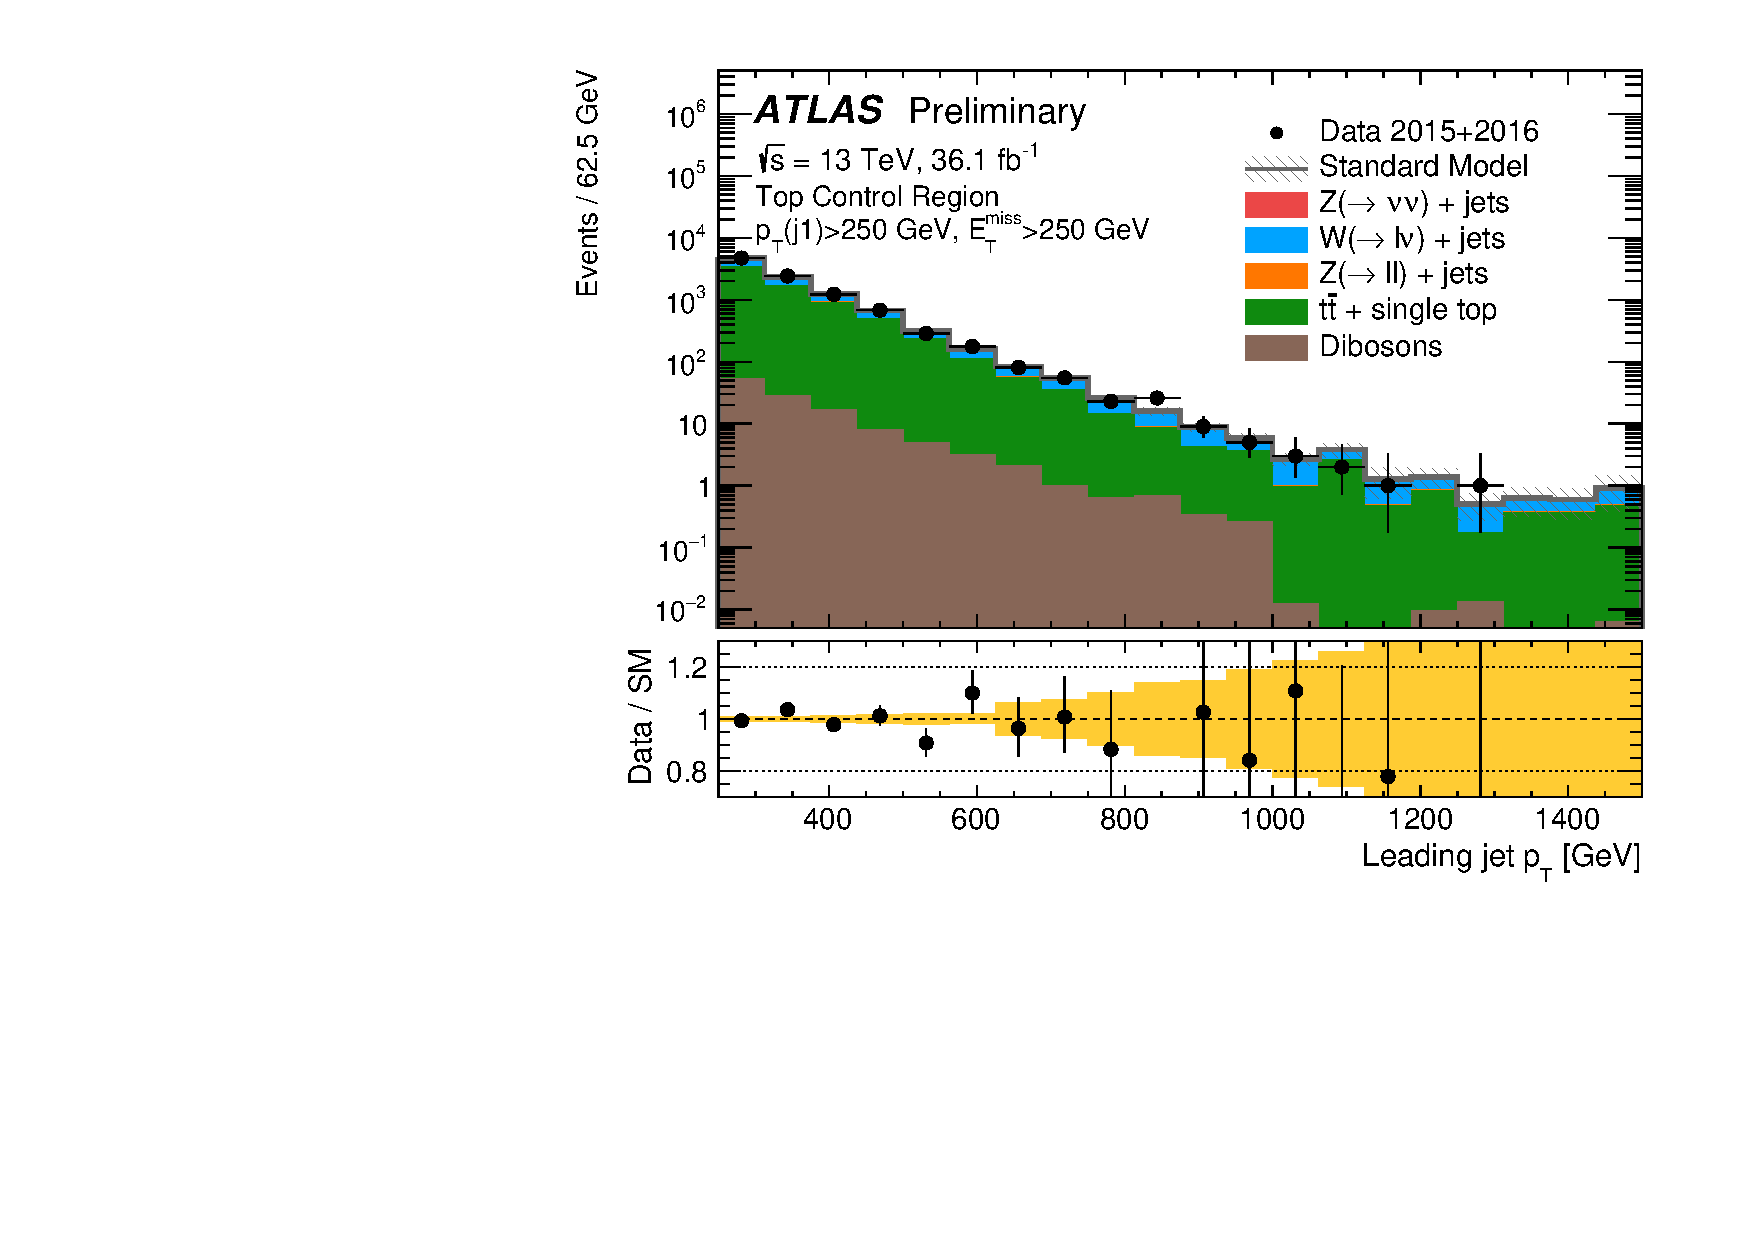
\includegraphics[width=\linewidth]{top_cr_jet1}
    \caption{Leading jet $\pt$ distribution.}
    \label{fig:top_cr_jet1}
  \end{subfigure}
  \caption{Observed and predicted $\met$ and leading jet $\pt$ after the
    background only fit in the $\crtop$ control region for the $\met > 250$~GeV
    inclusive selection. The error bands in the ratio plot on the bottom of the
    figures include statistical and systematic uncertainties. The negligible
    contribution of \gls{ncb} and diboson backgrounds is not reported in the
    figure.}
  \label{fig:top_plots}
\end{figure}
%%% Local Variables:
%%% mode: latex
%%% TeX-master: "../search_for_DM_LED_with_ATLAS"
%%% End:
